%% knit("quad-rig_catch_comparison.Rnw")

\documentclass[12pt]{article}\usepackage[]{graphicx}\usepackage[]{color}
%% maxwidth is the original width if it is less than linewidth
%% otherwise use linewidth (to make sure the graphics do not exceed the margin)
\makeatletter
\def\maxwidth{ %
  \ifdim\Gin@nat@width>\linewidth
    \linewidth
  \else
    \Gin@nat@width
  \fi
}
\makeatother

\definecolor{fgcolor}{rgb}{0.345, 0.345, 0.345}
\newcommand{\hlnum}[1]{\textcolor[rgb]{0.686,0.059,0.569}{#1}}%
\newcommand{\hlstr}[1]{\textcolor[rgb]{0.192,0.494,0.8}{#1}}%
\newcommand{\hlcom}[1]{\textcolor[rgb]{0.678,0.584,0.686}{\textit{#1}}}%
\newcommand{\hlopt}[1]{\textcolor[rgb]{0,0,0}{#1}}%
\newcommand{\hlstd}[1]{\textcolor[rgb]{0.345,0.345,0.345}{#1}}%
\newcommand{\hlkwa}[1]{\textcolor[rgb]{0.161,0.373,0.58}{\textbf{#1}}}%
\newcommand{\hlkwb}[1]{\textcolor[rgb]{0.69,0.353,0.396}{#1}}%
\newcommand{\hlkwc}[1]{\textcolor[rgb]{0.333,0.667,0.333}{#1}}%
\newcommand{\hlkwd}[1]{\textcolor[rgb]{0.737,0.353,0.396}{\textbf{#1}}}%

\usepackage{framed}
\makeatletter
\newenvironment{kframe}{%
 \def\at@end@of@kframe{}%
 \ifinner\ifhmode%
  \def\at@end@of@kframe{\end{minipage}}%
  \begin{minipage}{\columnwidth}%
 \fi\fi%
 \def\FrameCommand##1{\hskip\@totalleftmargin \hskip-\fboxsep
 \colorbox{shadecolor}{##1}\hskip-\fboxsep
     % There is no \\@totalrightmargin, so:
     \hskip-\linewidth \hskip-\@totalleftmargin \hskip\columnwidth}%
 \MakeFramed {\advance\hsize-\width
   \@totalleftmargin\z@ \linewidth\hsize
   \@setminipage}}%
 {\par\unskip\endMakeFramed%
 \at@end@of@kframe}
\makeatother

\definecolor{shadecolor}{rgb}{.97, .97, .97}
\definecolor{messagecolor}{rgb}{0, 0, 0}
\definecolor{warningcolor}{rgb}{1, 0, 1}
\definecolor{errorcolor}{rgb}{1, 0, 0}
\newenvironment{knitrout}{}{} % an empty environment to be redefined in TeX

\usepackage{alltt}
\usepackage{times}
\usepackage{hyperref}
\usepackage{natbib}
\hypersetup{pdfpagemode=UseNone} % don't show bookmarks on initial view
\hypersetup{colorlinks, urlcolor={blue}}

% revise margins
\setlength{\headheight}{0.0in}
\setlength{\topmargin}{0.0in}
\setlength{\headsep}{0.0in}
\setlength{\textheight}{8.65in}
\setlength{\footskip}{0.35in}
\setlength{\oddsidemargin}{0.0in}
\setlength{\evensidemargin}{0.0in}
\setlength{\textwidth}{6.5in}

\setlength{\parskip}{6pt}
\setlength{\parindent}{0pt}

\title{Preliminary multinomial analysis of \emph{Arkh Angell} data}
\author{For discussion}
\date{}
\IfFileExists{upquote.sty}{\usepackage{upquote}}{}
\begin{document}



\maketitle

\section{Data}

\begin{knitrout}\footnotesize
\definecolor{shadecolor}{rgb}{0.969, 0.969, 0.969}\color{fgcolor}\begin{kframe}
\begin{alltt}
\hlkwd{library}\hlstd{(gdata)}

\hlstd{arkh.neph.dat} \hlkwb{<-} \hlkwd{read.xls}\hlstd{(}\hlstr{"../data/2015 BIM Nephrops quad rig trials/Arkh Angell 70 V 100mm codends the Smalls 2015/Nephrops.xlsx"}\hlstd{,}
                     \hlkwc{sheet} \hlstd{=} \hlstr{"Nephrops length"}\hlstd{,}
                     \hlkwc{stringsAsFactors} \hlstd{=} \hlnum{FALSE}\hlstd{)}

\hlcom{## remove Haul 11 and 12 currently as these compare 80mm }
\hlstd{arkh.neph.dat} \hlkwb{<-} \hlkwd{subset}\hlstd{(arkh.neph.dat,} \hlopt{!}\hlstd{Haul} \hlopt \hlkwd{c}\hlstd{(}\hlnum{11}\hlstd{,} \hlnum{12}\hlstd{))}

\hlcom{## replace spaces in Compartment names}
\hlstd{arkh.neph.dat}\hlopt{$}\hlstd{Compartment} \hlkwb{<-} \hlkwd{gsub}\hlstd{(}\hlstr{" "}\hlstd{,} \hlstr{""}\hlstd{, arkh.neph.dat}\hlopt{$}\hlstd{Compartment)}

\hlcom{## remove any redundant levels}
\hlstd{arkh.neph.dat} \hlkwb{<-} \hlkwd{droplevels}\hlstd{(arkh.neph.dat)}

\hlcom{## Show the first 2 rows}
\hlkwd{head}\hlstd{(arkh.neph.dat,} \hlnum{2}\hlstd{)}

\hlcom{## Make the "HAUL" variable character}
\hlstd{arkh.neph.dat}\hlopt{$}\hlstd{HAUL} \hlkwb{<-} \hlkwd{paste}\hlstd{(}\hlstr{"H"}\hlstd{, arkh.neph.dat}\hlopt{$}\hlstd{Haul,} \hlkwc{sep} \hlstd{=}\hlstr{""}\hlstd{)}

\hlcom{## make some factor variables used in the analyses}
\hlstd{arkh.neph.dat}\hlopt{$}\hlstd{fHAUL} \hlkwb{<-} \hlkwd{factor}\hlstd{(arkh.neph.dat}\hlopt{$}\hlstd{HAUL,} \hlkwc{levels} \hlstd{=} \hlkwd{unique}\hlstd{(arkh.neph.dat}\hlopt{$}\hlstd{HAUL))}
\hlstd{arkh.neph.dat}\hlopt{$}\hlstd{Compartment} \hlkwb{<-} \hlkwd{factor}\hlstd{(}\hlkwd{paste}\hlstd{(}\hlstr{"c"}\hlstd{, arkh.neph.dat}\hlopt{$}\hlstd{Compartment,} \hlkwc{sep} \hlstd{=} \hlstr{""}\hlstd{))}

\hlcom{## remove observations above 99th and below 1th length percentile}
\hlcom{## these can be highly influential on the fits}
\hlstd{arkh.neph.dat} \hlkwb{<-} \hlkwd{subset}\hlstd{(arkh.neph.dat,}
                        \hlstd{Carapace.length} \hlopt{<} \hlkwd{quantile}\hlstd{(Carapace.length,} \hlnum{0.99}\hlstd{)} \hlopt{&}
                        \hlstd{Carapace.length} \hlopt{>} \hlkwd{quantile}\hlstd{(Carapace.length,} \hlnum{0.01}\hlstd{)}
                        \hlstd{)}
\end{alltt}
\end{kframe}
\end{knitrout}

Prepare the data for a multinomial fit.  

\begin{knitrout}\footnotesize
\definecolor{shadecolor}{rgb}{0.969, 0.969, 0.969}\color{fgcolor}\begin{kframe}
\begin{alltt}
\hlcom{## get count per length bin per haul by mesh size}
\hlcom{## using the reshape package (makes it easier to process data)}
\hlkwd{library}\hlstd{(reshape)}

\hlcom{## variables to keep }
\hlstd{vars2keep} \hlkwb{<-} \hlkwd{c}\hlstd{(}\hlstr{"Compartment"}\hlstd{,} \hlstr{"Carapace.length"}\hlstd{,} \hlstr{"fHAUL"}\hlstd{,} \hlstr{"Count"}\hlstd{)}

\hlcom{## melt the data frame}
\hlstd{arkh.neph.melt} \hlkwb{<-} \hlkwd{melt}\hlstd{(arkh.neph.dat[, vars2keep],}
                  \hlkwc{id} \hlstd{=} \hlkwd{c}\hlstd{(}\hlstr{"Compartment"}\hlstd{,} \hlstr{"Carapace.length"}\hlstd{,} \hlstr{"fHAUL"}\hlstd{))}

\hlcom{## re-form the dataframe in required format }
\hlstd{arkh.neph.cast} \hlkwb{<-} \hlkwd{cast}\hlstd{(arkh.neph.melt, Carapace.length} \hlopt{+} \hlstd{fHAUL} \hlopt{~} \hlstd{Compartment}  \hlopt{+} \hlstd{variable)}
\hlstd{arkh.neph.cast} \hlkwb{<-} \hlstd{arkh.neph.cast[}\hlkwd{order}\hlstd{(arkh.neph.cast}\hlopt{$}\hlstd{fHAUL,}
                                       \hlstd{arkh.neph.cast}\hlopt{$}\hlstd{Carapace.length), ]}
\hlstd{arkh.neph.cast[}\hlkwd{is.na}\hlstd{(arkh.neph.cast)]} \hlkwb{<-} \hlnum{0}

\hlcom{## show the first few rows}
\hlkwd{head}\hlstd{(arkh.neph.cast,} \hlnum{2}\hlstd{)}

\hlcom{## format the subsampling ratio similarly}

\hlcom{## multiple raising factors per haul}
\hlstd{rf.count} \hlkwb{<-} \hlkwd{with}\hlstd{(arkh.neph.dat,} \hlkwd{table}\hlstd{(fHAUL, Raising.factor, Compartment))}

\hlkwd{apply}\hlstd{(rf.count,} \hlnum{1}\hlstd{,} \hlkwc{FUN} \hlstd{=} \hlkwa{function}\hlstd{(}\hlkwc{x}\hlstd{)\{}\hlkwd{sum}\hlstd{(x}\hlopt{>}\hlnum{0}\hlstd{)\})}
\hlcom{## hauls 4 and 9}
\hlcom{## rf.count["H4",,] ## 6.8(28obs) and 6.9(2obs) for 100mm Port}
\hlcom{## rf.count["H9",,] ## 15.4(27obs) and 15.5(2obs) for 100mm Starboard}
\hlcom{## re-set}
\hlstd{arkh.neph.dat}\hlopt{$}\hlstd{Raising.factor[arkh.neph.dat}\hlopt{$}\hlstd{fHAUL} \hlopt{==} \hlstr{"H4"} \hlopt{&}
                             \hlstd{arkh.neph.dat}\hlopt{$}\hlstd{Compartment} \hlopt{==} \hlstr{"c100mmPort"}\hlstd{]} \hlkwb{<-} \hlnum{6.8}
\hlstd{arkh.neph.dat}\hlopt{$}\hlstd{Raising.factor[arkh.neph.dat}\hlopt{$}\hlstd{fHAUL} \hlopt{==} \hlstr{"H9"} \hlopt{&}
                             \hlstd{arkh.neph.dat}\hlopt{$}\hlstd{Compartment} \hlopt{==} \hlstr{"c100mmStarboard"}\hlstd{]} \hlkwb{<-} \hlnum{15.4}

\hlcom{## convert to sub-sampling ratio as in Celtic Warrior}
\hlstd{arkh.neph.dat}\hlopt{$}\hlstd{SUBSRATIO} \hlkwb{<-} \hlnum{1}\hlopt{/}\hlstd{arkh.neph.dat}\hlopt{$}\hlstd{Raising.factor}

\hlstd{vars2keep} \hlkwb{<-} \hlkwd{c}\hlstd{(}\hlstr{"Compartment"}\hlstd{,} \hlstr{"fHAUL"}\hlstd{,} \hlstr{"SUBSRATIO"}\hlstd{)}

\hlstd{subs.melt} \hlkwb{<-} \hlkwd{melt}\hlstd{(}\hlkwd{unique}\hlstd{(arkh.neph.dat[, vars2keep]),} \hlkwc{id} \hlstd{=} \hlkwd{c}\hlstd{(}\hlstr{"Compartment"}\hlstd{,} \hlstr{"fHAUL"}\hlstd{))}

\hlstd{subs.cast} \hlkwb{<-} \hlkwd{cast}\hlstd{(subs.melt, fHAUL}  \hlopt{~} \hlstd{Compartment} \hlopt{+} \hlstd{variable)}

\hlcom{## merge counts and subsampling ratio back together }
\hlstd{arkh.neph.cast} \hlkwb{<-} \hlkwd{merge}\hlstd{(arkh.neph.cast, subs.cast,} \hlkwc{by} \hlstd{=} \hlstr{"fHAUL"}\hlstd{,} \hlkwc{all.x} \hlstd{=} \hlnum{TRUE}\hlstd{)}

\hlcom{## show first few lines}
\hlkwd{head}\hlstd{(arkh.neph.cast,} \hlnum{2}\hlstd{)}

\hlcom{## Extract the matrix of counts}
\hlstd{count.vars} \hlkwb{<-} \hlkwd{c}\hlstd{(}\hlstr{"c100mmPort_Count"}\hlstd{,} \hlstr{"c70mmPort_Count"}\hlstd{,}
                \hlstr{"c100mmStarboard_Count"}\hlstd{,} \hlstr{"c70mmStarboard_Count"}\hlstd{)}

\hlstd{neph.count.mat} \hlkwb{<-} \hlkwd{as.matrix}\hlstd{(arkh.neph.cast[, count.vars])}

\hlkwd{colnames}\hlstd{(neph.count.mat)} \hlkwb{<-} \hlkwd{c}\hlstd{(}\hlstr{"c100mmPort_Count"}\hlstd{,} \hlstr{"c70mmPort_Count"}\hlstd{,}
                              \hlstr{"c100mmStarboard_Count"}\hlstd{,} \hlstr{"c70mmStarboard_Count"}\hlstd{)}

\hlcom{## Extract the matrix of subsampling ratios}
\hlstd{subsratio.vars} \hlkwb{<-} \hlkwd{c}\hlstd{(}\hlstr{"c100mmPort_SUBSRATIO"}\hlstd{,} \hlstr{"c70mmPort_SUBSRATIO"}\hlstd{,}
                    \hlstr{"c100mmStarboard_SUBSRATIO"}\hlstd{,} \hlstr{"c70mmStarboard_SUBSRATIO"}\hlstd{)}

\hlstd{subsratio.mat} \hlkwb{<-} \hlkwd{as.matrix}\hlstd{(arkh.neph.cast[, subsratio.vars])}

\hlcom{## Create the offset (NEED TO CHECK THIS)}
\hlstd{offset.mat} \hlkwb{<-} \hlkwd{log}\hlstd{(}\hlkwd{apply}\hlstd{(subsratio.mat,} \hlnum{2}\hlstd{,} \hlkwc{FUN} \hlstd{=}
                        \hlkwa{function}\hlstd{(}\hlkwc{zz}\hlstd{)\{zz}\hlopt{/}\hlstd{subsratio.mat[,}\hlnum{1}\hlstd{]\}))}
\end{alltt}
\end{kframe}
\end{knitrout}

Plot the data 
\begin{knitrout}\footnotesize
\definecolor{shadecolor}{rgb}{0.969, 0.969, 0.969}\color{fgcolor}\begin{kframe}
\begin{alltt}
\hlkwd{library}\hlstd{(ggplot2)}

\hlcom{## Get the proportions}
\hlstd{count.mesh} \hlkwb{<-} \hlkwd{as.matrix}\hlstd{(arkh.neph.cast[, count.vars])}

\hlstd{prop.mesh} \hlkwb{<-} \hlkwd{prop.table}\hlstd{(count.mesh,} \hlkwc{margin} \hlstd{=} \hlnum{1}\hlstd{)}

\hlstd{m} \hlkwb{<-} \hlkwd{dim}\hlstd{(prop.mesh)[}\hlnum{1}\hlstd{]}

\hlcom{## make a dataframe of the proportions for ggplot}
\hlstd{prop.mesh.df} \hlkwb{<-} \hlkwd{data.frame}\hlstd{(}
                  \hlkwc{Mesh.Size} \hlstd{=} \hlkwd{factor}\hlstd{(}\hlkwd{rep}\hlstd{(}
                    \hlkwd{c}\hlstd{(}\hlstr{"100mmPort"}\hlstd{,} \hlstr{"70mmPort"}\hlstd{,} \hlstr{"100mmStarboard"}\hlstd{,} \hlstr{"70mmStarboard"}\hlstd{),}
                    \hlkwc{each} \hlstd{= m),}
                    \hlkwc{levels} \hlstd{=} \hlkwd{c}\hlstd{(}\hlstr{"100mmPort"}\hlstd{,} \hlstr{"70mmPort"}\hlstd{,} \hlstr{"100mmStarboard"}\hlstd{,} \hlstr{"70mmStarboard"}\hlstd{)),}
                  \hlkwc{Carapace.length} \hlstd{=} \hlkwd{rep}\hlstd{(arkh.neph.cast}\hlopt{$}\hlstd{Carapace.length,} \hlkwc{times} \hlstd{=} \hlnum{4}\hlstd{),}
                  \hlkwc{fHAUL} \hlstd{=} \hlkwd{rep}\hlstd{(arkh.neph.cast}\hlopt{$}\hlstd{fHAUL,} \hlkwc{times} \hlstd{=} \hlnum{4}\hlstd{),}
                  \hlkwc{proportion} \hlstd{=} \hlkwd{c}\hlstd{(prop.mesh),}
                  \hlkwc{count} \hlstd{=} \hlkwd{c}\hlstd{(count.mesh))}

\hlkwd{ggplot}\hlstd{(prop.mesh.df,} \hlkwd{aes}\hlstd{(}\hlkwc{x} \hlstd{= Carapace.length,} \hlkwc{y} \hlstd{= proportion))} \hlopt{+}
  \hlkwd{geom_point}\hlstd{(}\hlkwc{colour} \hlstd{=} \hlstr{"#F8766D"}\hlstd{,} \hlkwc{alpha} \hlstd{=} \hlnum{0.2}\hlstd{,} \hlkwd{aes}\hlstd{(}\hlkwc{size} \hlstd{=} \hlkwd{log}\hlstd{(count)))} \hlopt{+}
  \hlkwd{facet_wrap}\hlstd{(}\hlopt{~} \hlstd{Mesh.Size)} \hlopt{+} \hlkwd{ylab}\hlstd{(}\hlstr{"Proportion of Nephrops per cod-end"}\hlstd{)}
\end{alltt}
\end{kframe}\begin{figure}
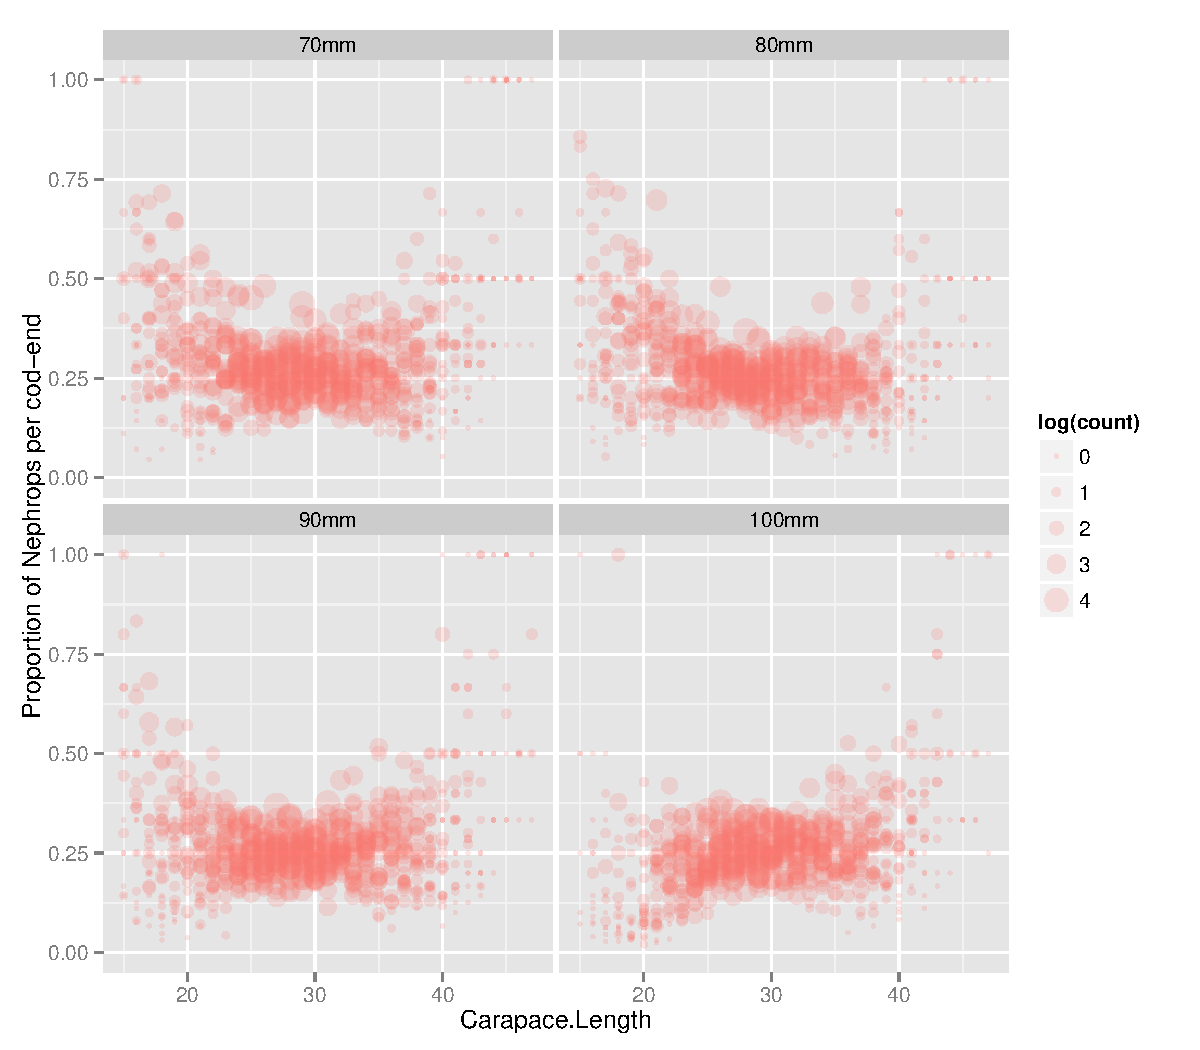
\includegraphics[width=\maxwidth]{figure/unnamed-chunk-4-1} \caption[Arkh Angell quad-rig trial]{Arkh Angell quad-rig trial. Proportion of Nephrops catch retained per haul. Each point represents the proportion of the Nephrops catch (in number) per haul and length class retained in a given cod-end (70mm, 80mm, 90mm, or 100mm). The size of the point is proportional to the log of the count.}\label{fig:unnamed-chunk-4}
\end{figure}


\end{knitrout}

\section{Model}
The model we focus on is the multinomial, which is a generalization of the binomial to cases with more than two categories (here 4 categories: 100mm Port, 70mm Port, 100mm Starboard, 70mm Starboard). Under the assumption that each net fishes the same, we would expect 25\% of the catch to be retained in each net. We can test that hypothesis.

\begin{knitrout}\footnotesize
\definecolor{shadecolor}{rgb}{0.969, 0.969, 0.969}\color{fgcolor}\begin{kframe}
\begin{alltt}
\hlkwd{library}\hlstd{(nnet)}

\hlcom{## First fit is constant proportions}
\hlcom{## not accounting for length}

\hlstd{mnom0} \hlkwb{<-} \hlkwd{multinom}\hlstd{(neph.count.mat} \hlopt{~} \hlnum{1}\hlstd{)}

\hlcom{## include carapace length }
\hlcom{## first scale it to range between zero and one}
\hlstd{max.length} \hlkwb{<-} \hlkwd{max}\hlstd{(arkh.neph.cast}\hlopt{$}\hlstd{Carapace.length)}
\hlstd{arkh.neph.cast}\hlopt{$}\hlstd{prop.Carapace.length} \hlkwb{<-} \hlstd{arkh.neph.cast}\hlopt{$}\hlstd{Carapace.length}\hlopt{/}\hlstd{max.length}

\hlcom{## Extend to third order polynomial (based on AIC and BIC)}
\hlstd{arkh.neph.cast}\hlopt{$}\hlstd{prop.Carapace.length2} \hlkwb{<-} \hlstd{arkh.neph.cast}\hlopt{$}\hlstd{prop.Carapace.length}\hlopt{^}\hlnum{2}
\hlstd{arkh.neph.cast}\hlopt{$}\hlstd{prop.Carapace.length3} \hlkwb{<-} \hlstd{arkh.neph.cast}\hlopt{$}\hlstd{prop.Carapace.length}\hlopt{^}\hlnum{3}

\hlcom{## }
\hlstd{mnom.length} \hlkwb{<-} \hlkwd{multinom}\hlstd{(neph.count.mat} \hlopt{~}
                        \hlstd{prop.Carapace.length} \hlopt{+} \hlstd{prop.Carapace.length2} \hlopt{+}
                        \hlstd{prop.Carapace.length3,} \hlkwc{data} \hlstd{= arkh.neph.cast)}

\hlkwd{AIC}\hlstd{(mnom0, mnom.length)}

\hlcom{## try a VGAM fit for comparison}
\hlcom{## particularly for 100mm Port small lengths}
\hlkwd{library}\hlstd{(VGAM)}

\hlcom{## find out best degrees of freedom}
\hlstd{df.vec} \hlkwb{<-} \hlkwd{seq}\hlstd{(}\hlnum{1}\hlstd{,}\hlnum{10}\hlstd{)}
\hlstd{aic.vec} \hlkwb{<-} \hlkwd{rep}\hlstd{(}\hlnum{NA}\hlstd{,} \hlnum{10}\hlstd{)}

\hlkwa{for}\hlstd{(i} \hlkwa{in} \hlnum{1}\hlopt{:}\hlnum{10}\hlstd{)\{}
  \hlstd{mnom.length.vgam} \hlkwb{<-} \hlkwd{vgam}\hlstd{(neph.count.mat} \hlopt{~}
                           \hlkwd{s}\hlstd{(prop.Carapace.length,} \hlkwc{df} \hlstd{= df.vec[i]),}
                           \hlkwc{family} \hlstd{= multinomial,} \hlkwc{data} \hlstd{= arkh.neph.cast)}
  \hlstd{aic.vec[i]} \hlkwb{<-} \hlkwd{AIC}\hlstd{(mnom.length.vgam)}
\hlstd{\}}

\hlstd{df.best} \hlkwb{<-} \hlstd{df.vec[}\hlkwd{which.min}\hlstd{(aic.vec)]}
\hlstd{mnom.length.vgam} \hlkwb{<-} \hlkwd{vgam}\hlstd{(neph.count.mat} \hlopt{~}
                         \hlkwd{s}\hlstd{(prop.Carapace.length,} \hlkwc{df} \hlstd{= df.best),}
                         \hlkwc{family} \hlstd{= multinomial,} \hlkwc{data} \hlstd{= arkh.neph.cast)}

\hlstd{pred.prop.length} \hlkwb{<-} \hlkwd{seq}\hlstd{(}\hlkwd{min}\hlstd{(arkh.neph.cast}\hlopt{$}\hlstd{prop.Carapace.length),}
                        \hlkwd{max}\hlstd{(arkh.neph.cast}\hlopt{$}\hlstd{prop.Carapace.length),} \hlkwc{length} \hlstd{=} \hlnum{100}\hlstd{)}

\hlstd{pred.length} \hlkwb{<-} \hlkwd{seq}\hlstd{(}\hlkwd{min}\hlstd{(arkh.neph.cast}\hlopt{$}\hlstd{Carapace.length),}
                        \hlkwd{max}\hlstd{(arkh.neph.cast}\hlopt{$}\hlstd{Carapace.length),} \hlkwc{length} \hlstd{=} \hlnum{100}\hlstd{)}

\hlstd{pred.vgam} \hlkwb{<-} \hlkwd{predict}\hlstd{(mnom.length.vgam,}
                     \hlkwc{newdata} \hlstd{=} \hlkwd{data.frame}\hlstd{(}\hlkwc{prop.Carapace.length} \hlstd{= pred.prop.length),}
                     \hlkwc{type} \hlstd{=} \hlstr{"response"}\hlstd{)}

\hlstd{pred.vgam.df} \hlkwb{<-} \hlkwd{data.frame}\hlstd{(}
                  \hlkwc{Mesh.Size} \hlstd{=}
                  \hlkwd{factor}\hlstd{(}\hlkwd{rep}\hlstd{(}\hlkwd{c}\hlstd{(}\hlstr{"100mmPort"}\hlstd{,} \hlstr{"70mmPort"}\hlstd{,}
                               \hlstr{"100mmStarboard"}\hlstd{,} \hlstr{"70mmStarboard"}\hlstd{),}
                    \hlkwc{each} \hlstd{= m),}
                         \hlkwc{levels} \hlstd{=} \hlkwd{c}\hlstd{(}\hlstr{"100mmPort"}\hlstd{,} \hlstr{"70mmPort"}\hlstd{,}
                           \hlstr{"100mmStarboard"}\hlstd{,} \hlstr{"70mmStarboard"}\hlstd{)),}
                  \hlkwc{Carapace.length} \hlstd{=} \hlkwd{rep}\hlstd{(pred.length,} \hlkwc{times} \hlstd{=} \hlnum{4}\hlstd{),}
                  \hlkwc{proportion} \hlstd{=} \hlkwd{c}\hlstd{(pred.vgam))}
\end{alltt}
\end{kframe}
\end{knitrout}

Get predictions for the fitted model (note this is long-winded here but will be better coded for more than the preliminary example).

\begin{knitrout}\footnotesize
\definecolor{shadecolor}{rgb}{0.969, 0.969, 0.969}\color{fgcolor}\begin{kframe}
\begin{alltt}
\hlcom{## get predictions manually}
\hlcom{## CIs not defined in multinomial context but let's try}

\hlcom{## fit coefficients}
\hlstd{beta.mu} \hlkwb{<-} \hlkwd{c}\hlstd{(}\hlkwd{t}\hlstd{(}\hlkwd{coef}\hlstd{(mnom.length)))}

\hlcom{## fit coefficient variance covariance matrix}
\hlstd{Sigma} \hlkwb{<-} \hlkwd{vcov}\hlstd{(mnom.length)}

\hlcom{## number of lengths to predict for}
\hlstd{nlength} \hlkwb{<-} \hlnum{100}
\hlstd{pred.prop.length} \hlkwb{<-} \hlkwd{seq}\hlstd{(}\hlkwd{min}\hlstd{(arkh.neph.cast}\hlopt{$}\hlstd{prop.Carapace.length),}
                        \hlkwd{max}\hlstd{(arkh.neph.cast}\hlopt{$}\hlstd{prop.Carapace.length),} \hlkwc{length} \hlstd{=} \hlnum{100}\hlstd{)}

\hlstd{pred.length} \hlkwb{<-} \hlkwd{seq}\hlstd{(}\hlkwd{min}\hlstd{(arkh.neph.cast}\hlopt{$}\hlstd{Carapace.length),}
                        \hlkwd{max}\hlstd{(arkh.neph.cast}\hlopt{$}\hlstd{Carapace.length),} \hlkwc{length} \hlstd{=} \hlnum{100}\hlstd{)}

\hlcom{## model matrix}
\hlstd{X} \hlkwb{<-} \hlkwd{cbind}\hlstd{(}\hlnum{1}\hlstd{, pred.prop.length, pred.prop.length}\hlopt{^}\hlnum{2}\hlstd{, pred.prop.length}\hlopt{^}\hlnum{3}\hlstd{)}

\hlcom{## number of times to resample predictions to get CIs}
\hlstd{nresamp} \hlkwb{<-} \hlnum{100}
\hlstd{pred.array} \hlkwb{<-} \hlkwd{array}\hlstd{(}\hlnum{NA}\hlstd{,} \hlkwc{dim} \hlstd{=} \hlkwd{c}\hlstd{(nlength,} \hlnum{4}\hlstd{, nresamp))}

\hlcom{## package to draw from multivariate normal }
\hlkwd{library}\hlstd{(mvtnorm)}

\hlkwa{for}\hlstd{(i} \hlkwa{in} \hlnum{1}\hlopt{:}\hlstd{nresamp)\{}
  \hlcom{## print(i)}
  \hlstd{beta} \hlkwb{<-} \hlkwd{matrix}\hlstd{(}\hlkwd{rmvnorm}\hlstd{(}\hlnum{1}\hlstd{,} \hlkwc{mean} \hlstd{= beta.mu,} \hlkwc{sigma} \hlstd{= Sigma),}
                 \hlkwc{nrow} \hlstd{=} \hlnum{3}\hlstd{,} \hlkwc{byrow} \hlstd{=} \hlnum{TRUE}\hlstd{)}
  \hlstd{p70mmPort} \hlkwb{<-} \hlkwd{exp}\hlstd{(X} \hlopt \hlkwd{matrix}\hlstd{(beta[}\hlnum{1}\hlstd{,]))}\hlopt{/}\hlstd{(}\hlnum{1} \hlopt{+} \hlkwd{rowSums}\hlstd{(}\hlkwd{exp}\hlstd{(X} \hlopt \hlkwd{t}\hlstd{(beta))))}
  \hlstd{p100mmStarboard} \hlkwb{<-} \hlkwd{exp}\hlstd{(X} \hlopt \hlkwd{matrix}\hlstd{(beta[}\hlnum{2}\hlstd{,]))}\hlopt{/}\hlstd{(}\hlnum{1} \hlopt{+} \hlkwd{rowSums}\hlstd{(}\hlkwd{exp}\hlstd{(X} \hlopt \hlkwd{t}\hlstd{(beta))))}
  \hlstd{p70mmStarboard} \hlkwb{<-} \hlkwd{exp}\hlstd{(X} \hlopt \hlkwd{matrix}\hlstd{(beta[}\hlnum{3}\hlstd{,]))}\hlopt{/}\hlstd{(}\hlnum{1} \hlopt{+} \hlkwd{rowSums}\hlstd{(}\hlkwd{exp}\hlstd{(X} \hlopt \hlkwd{t}\hlstd{(beta))))}
  \hlstd{p100mmPort} \hlkwb{<-} \hlnum{1} \hlopt{-} \hlstd{p70mmPort} \hlopt{-} \hlstd{p100mmStarboard} \hlopt{-} \hlstd{p70mmStarboard}
  \hlstd{pred.p} \hlkwb{<-} \hlkwd{cbind}\hlstd{(p100mmPort, p70mmPort, p100mmStarboard, p70mmStarboard)}
  \hlstd{pred.array[ , , i]} \hlkwb{<-} \hlstd{pred.p}
  \hlkwd{rm}\hlstd{(pred.p)}
\hlstd{\}}

\hlcom{## mean across samples}
\hlstd{pred.mu} \hlkwb{<-} \hlkwd{apply}\hlstd{(pred.array,} \hlkwd{c}\hlstd{(}\hlnum{1}\hlstd{,} \hlnum{2}\hlstd{), mean)}

\hlcom{## upper across samples}
\hlstd{pred.upper} \hlkwb{<-} \hlkwd{apply}\hlstd{(pred.array,} \hlkwd{c}\hlstd{(}\hlnum{1}\hlstd{,} \hlnum{2}\hlstd{), quantile,} \hlkwc{p} \hlstd{=} \hlnum{0.975}\hlstd{)}

\hlcom{## lower across samples}
\hlstd{pred.lower} \hlkwb{<-} \hlkwd{apply}\hlstd{(pred.array,} \hlkwd{c}\hlstd{(}\hlnum{1}\hlstd{,} \hlnum{2}\hlstd{), quantile,} \hlkwc{p} \hlstd{=} \hlnum{0.025}\hlstd{)}

\hlcom{## bring all together in a data frame for ggplot}
\hlstd{m} \hlkwb{<-} \hlkwd{dim}\hlstd{(pred.mu)[}\hlnum{1}\hlstd{]}

\hlstd{pred.ci.df} \hlkwb{<-} \hlkwd{data.frame}\hlstd{(}
                \hlkwc{Mesh.Size} \hlstd{=} \hlkwd{factor}\hlstd{(}\hlkwd{rep}\hlstd{(}\hlkwd{c}\hlstd{(}\hlstr{"100mmPort"}\hlstd{,} \hlstr{"70mmPort"}\hlstd{,}
                  \hlstr{"100mmStarboard"}\hlstd{,} \hlstr{"70mmStarboard"}\hlstd{),}
                 \hlkwc{each} \hlstd{= m),} \hlkwc{levels} \hlstd{=} \hlkwd{c}\hlstd{(}\hlstr{"100mmPort"}\hlstd{,} \hlstr{"70mmPort"}\hlstd{,}
                              \hlstr{"100mmStarboard"}\hlstd{,} \hlstr{"70mmStarboard"}\hlstd{)),}
                \hlkwc{Carapace.length} \hlstd{=} \hlkwd{rep}\hlstd{(pred.length,} \hlkwc{times} \hlstd{=} \hlnum{4}\hlstd{),}
                \hlkwc{proportion} \hlstd{=} \hlkwd{c}\hlstd{(pred.mu),}
                \hlkwc{lower} \hlstd{=} \hlkwd{c}\hlstd{(pred.lower),}
                \hlkwc{upper} \hlstd{=} \hlkwd{c}\hlstd{(pred.upper))}
\end{alltt}
\end{kframe}
\end{knitrout}

Finally overlay the fit on the sample proportions

\begin{knitrout}\footnotesize
\definecolor{shadecolor}{rgb}{0.969, 0.969, 0.969}\color{fgcolor}\begin{kframe}
\begin{alltt}
\hlstd{p} \hlkwb{<-} \hlkwd{ggplot}\hlstd{(prop.mesh.df,} \hlkwd{aes}\hlstd{(}\hlkwc{x} \hlstd{= Carapace.length,} \hlkwc{y} \hlstd{= proportion))} \hlopt{+}
  \hlkwd{geom_point}\hlstd{(}\hlkwc{colour} \hlstd{=} \hlstr{"#F8766D"}\hlstd{,} \hlkwc{alpha} \hlstd{=} \hlnum{0.2}\hlstd{,} \hlkwd{aes}\hlstd{(}\hlkwc{size} \hlstd{=} \hlkwd{log}\hlstd{(count)))} \hlopt{+}
\hlkwd{facet_wrap}\hlstd{(}\hlopt{~} \hlstd{Mesh.Size)} \hlopt{+} \hlkwd{ylab}\hlstd{(}\hlstr{"Proportion of Nephrops per cod-end"}\hlstd{)}

\hlstd{p} \hlopt{+} \hlkwd{geom_ribbon}\hlstd{(}\hlkwc{data}\hlstd{=pred.ci.df,} \hlkwd{aes}\hlstd{(}\hlkwc{ymin} \hlstd{= lower,} \hlkwc{ymax} \hlstd{= upper),}
                \hlkwc{alpha}\hlstd{=}\hlnum{0.3}\hlstd{,} \hlkwc{fill} \hlstd{=} \hlstr{"blue"}\hlstd{)} \hlopt{+}
  \hlkwd{geom_line}\hlstd{(}\hlkwc{data} \hlstd{= pred.ci.df,} \hlkwd{aes}\hlstd{(}\hlkwc{x} \hlstd{= Carapace.length,} \hlkwc{y} \hlstd{= proportion),}
            \hlkwc{col} \hlstd{=} \hlstr{"navy"}\hlstd{,} \hlkwc{size} \hlstd{=} \hlnum{0.5}\hlstd{)} \hlopt{+}
  \hlkwd{geom_hline}\hlstd{(}\hlkwd{aes}\hlstd{(}\hlkwc{yintercept} \hlstd{=} \hlnum{0.25}\hlstd{),} \hlkwc{linetype} \hlstd{=} \hlstr{"dashed"}\hlstd{)} \hlopt{+}
  \hlkwd{geom_line}\hlstd{(}\hlkwc{data} \hlstd{= pred.vgam.df,} \hlkwd{aes}\hlstd{(}\hlkwc{x} \hlstd{= Carapace.length,} \hlkwc{y} \hlstd{= proportion),}
            \hlkwc{col} \hlstd{=} \hlstr{"green"}\hlstd{,} \hlkwc{size} \hlstd{=} \hlnum{0.5}\hlstd{)}
\end{alltt}
\end{kframe}\begin{figure}
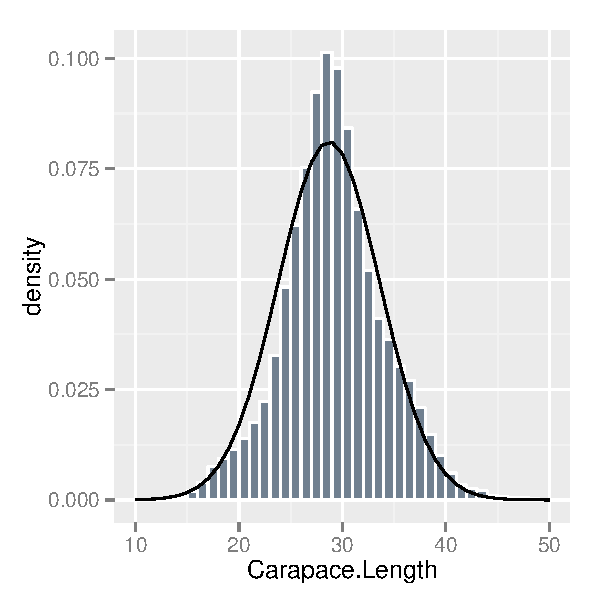
\includegraphics[width=\maxwidth]{figure/unnamed-chunk-7-1} \caption[Arkh Angell quad-rig trials]{Arkh Angell quad-rig trials. Proportion of Nephrops catch retained per haul with fitted multinomial model and associated re-sampled intervals (blue). Null hypothesis of equal retention is displayed as the dashed line at 0.25. A multinomial additive model is shown in green for comparison.}\label{fig:unnamed-chunk-7}
\end{figure}


\end{knitrout}

\bibliography{../../../../misc/epif_bibliography}
\bibliographystyle{../../../../misc/cjfas}
\end{document}

